\documentclass[a4paper,12pt]{article}

\usepackage{geometry}
\geometry{left=2cm, right=2cm, top=2cm, bottom=2cm}


\usepackage[english,russian]{babel}
\usepackage[T2A]{fontenc}
\usepackage[utf8]{inputenc}

\usepackage{amsmath,amsfonts,amssymb,amsthm,mathtools}
\usepackage[]{hyperref}

\usepackage{float}

\renewenvironment{itemize}{
    \begin{list}{\labelitemi}{
    \setlength{\topsep}{0pt}
    \setlength{\partopsep}{6pt}
    \setlength{\parskip}{0pt}
    \setlength{\itemsep}{0pt}
    \setlength{\parsep}{0pt}
    }
}{\end{list}}

%https://en.wikibooks.org/wiki/LaTeX/Title_Creation

\author{Быковских~Д.А.}
\title{
    Компьютерная графика \\ 
    Лабораторная работа №0. \\ 
    Настройка ИСР на примере VSCodium для Windows
    }
\date{сентябрь 2023 г.}

\begin{document}
        
\fontsize{14pt}{16pt}\selectfont

    \maketitle

   \section{Введение}
        Данная инструкция содержит подробное описание установки и настройки интегрированной среды разработки (ИСР или IDE) на примере ИСР VSCodium (далее VSCodium), а также других вспомогательных инструментов и приложений, необходимых для успешной разработки ваших приложений по дисциплине \textquotedbl Компьютерная графика\textquotedbl, включая компиляцию, запуск и отладку. Эту инструкцию можно также использовать для установки и настройки Visual~Studio~Code (VS~Code) или Code~--~OSS.
        
        \underline{Следует подчеркнуть}, что на сегодняшний день мне \textbf{неизвестен} способ корректной работы приложений, использующих графические библиотеки, \textbf{в виртуальной машине}. (Если у кого-то вдруг получится, я готов перенять опыт.)
        
    \section{Настройка ИСР}

        Для того чтобы разрабатывать программы под ОС семейства MS Windows (далее Windows) необходимо выполнить ниже описанные шаги.
        
        \subsection{Установка среды MSYS2}

        MSYS2 --- среда разработки и исполнения программ для Windows. Она включает в себя командную оболочку и утилиты, которые позволяют разработчикам работать с программами и библиотеками, предназначенными для Unix-подобных операционных систем, под управлением Windows.

        Перейдите по \href{https://www.msys2.org/}{ссылке} и скачайте установочный файл, установите MSYS2 (там даже показано, как устанавливать пакеты).
    
        
        \subsection{Установка с помощью командной оболочки MSYS2 необходимых библиотек, компиляторов и др.}

        После установки запустите командную оболочку (terminal) MSYS2, обновите и установите пакеты, введя следующие команды:
        
        \begin{itemize}
            \item[] pacman -Syu --noconfirm
            \item[] pacman -S --noconfirm mingw-w64-x86\_64-gcc
            \item[] pacman -S --noconfirm mingw-w64-x86\_64-gdb
            \item[] pacman -S --noconfirm mingw-w64-x86\_64-cmake
            \item[] pacman -S --noconfirm mingw-w64-x86\_64-glfw
            \item[] pacman -S --noconfirm mingw-w64-x86\_64-glew
            \item[] pacman -S --noconfirm mingw-w64-x86\_64-assimp
            \item[] pacman -S --noconfirm mingw-w64-x86\_64-glm
            \item[] pacman -S --noconfirm mingw-w64-x86\_64-soil

        \end{itemize}
                
        Обратите внимание, что первая строка связана с обновлением. Возможно, потребуется ее выполнить еще раз, поскольку в процессе обновления может быть необходим перезапуск командной оболочки, прежде чем действительно установятся все обновления.

        %В случае, если rm /var/lib/pacman/db.lck

        %Посмотреть, как устанавливать пакеты, можно \href{https://www.msys2.org/}{здесь}.

        Примечание. 
        По умолчанию исполняемые бинарные файлы, имеющие расширение exe, находятся в директории \textquotedbl C:\textbackslash msys64\textbackslash mingw64\textbackslash bin\textquotedbl. Говоря в целом, библиотеки, заголовочные файлы и пр. расположены в поддиректориях директории \textquotedbl C:\textbackslash msys64\textbackslash mingw64\textquotedbl.

        \subsection{Установка VSCodium}
        
        Скачайте с \href{https://github.com/VSCodium/vscodium/releases/}{официального сайта} установочный файл, имеющий расширение msi или exe, и установите VSCodium.

        Примечание.       
        Эта ИСР --- аналог VS~Code, является свободной и не передает стороннюю информацию (например, телеметрию) компании Microsoft. 
        
        \subsection{Установка расширений для VSCodium}
        
        Запустите VSCodium и перейдите на вкладку Extensions (расширения) с помощью комбинации клавиш Ctrl+Shift+X, чтобы установить расширения.
        
        Теперь установите следующие расширения (см. рис.~\ref{fig:installed_extensions}):

        \begin{itemize}
            \item MSYS2/Cygwin/MinGW/Clang support;
            \item CMake Tools;
            \item CMake;
            \item C/C++ (\href{https://marketplace.visualstudio.com/items?itemName=ms-vscode.cpptools}{ссылка});
            \item glsl-canvas (\href{https://marketplace.visualstudio.com/items?itemName=circledev.glsl-canvas}{ссылка});
            \item Shader languages support for VS Code;
            \item vscode-pdf.
        \end{itemize}

        Недостающие расширения, т.е. VSIX файлы, можно найти на \href{https://marketplace.visualstudio.com/vscode}{официальном сайте Marketplace}, где размещаются расширения.
        
        \begin{figure}[H]
            \centering
			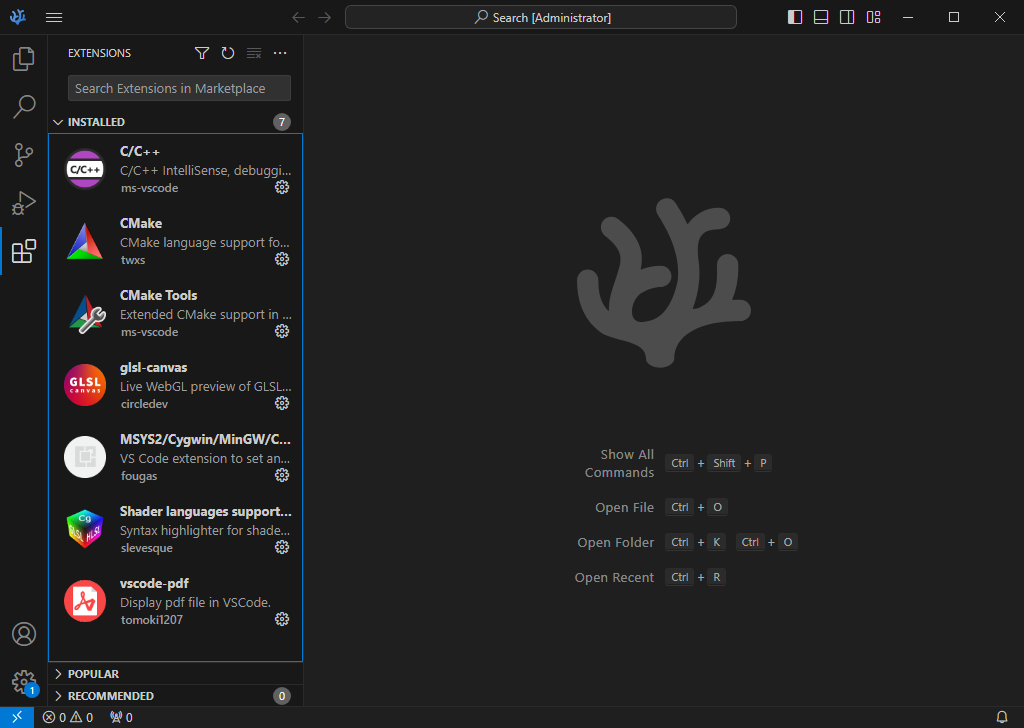
\includegraphics[width=0.85\textwidth]{images/Installed_extenstions.png}
			\caption {Отображение установленных расширений}
            \label{fig:installed_extensions}
        \end{figure}
        
        Например, чтобы установить glsl-canvas расширение, необходимо скачать VSIX файл, а для этого необходимо кликнуть на ссылку \textquotedbl Download Extension\textquotedbl \ на \href{https://marketplace.visualstudio.com/items?itemName=circledev.glsl-canvas}{странице сайта} (см. правый нижний угол рис.~\ref{fig:Downloading_glsl-canvas}).


        \begin{figure}[H]
            \centering
			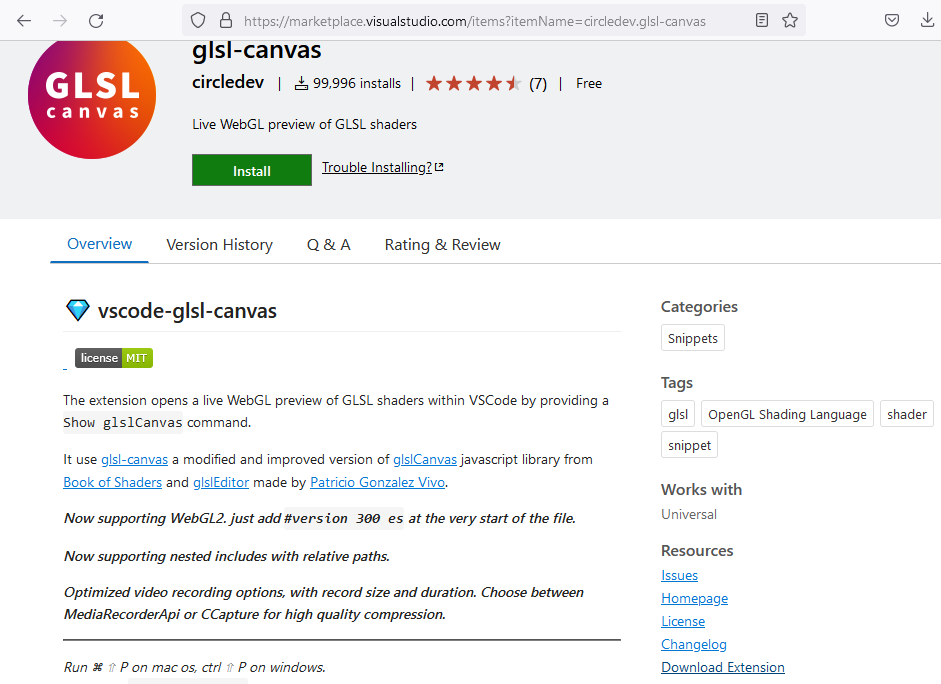
\includegraphics[width=0.85\textwidth]{images/Downloading_glsl-canvas.png}
			\caption {Скачивание glsl-canvas расширения}
            \label{fig:Downloading_glsl-canvas}
        \end{figure}


        Некоторые расширения, после их скачивания, можно установить следующим образом. На панели в правом верхнем углу необходимо навести курсор на \textquotedbl 3 точки\textquotedbl \ и нажать клавишу мыши, после выбрать пункт \textquotedbl Install~from~VSIX\textquotedbl \\ (см. рис.~\ref{fig:installing_downloaded_extensions}).
        


        \begin{figure}[H]
            \centering
			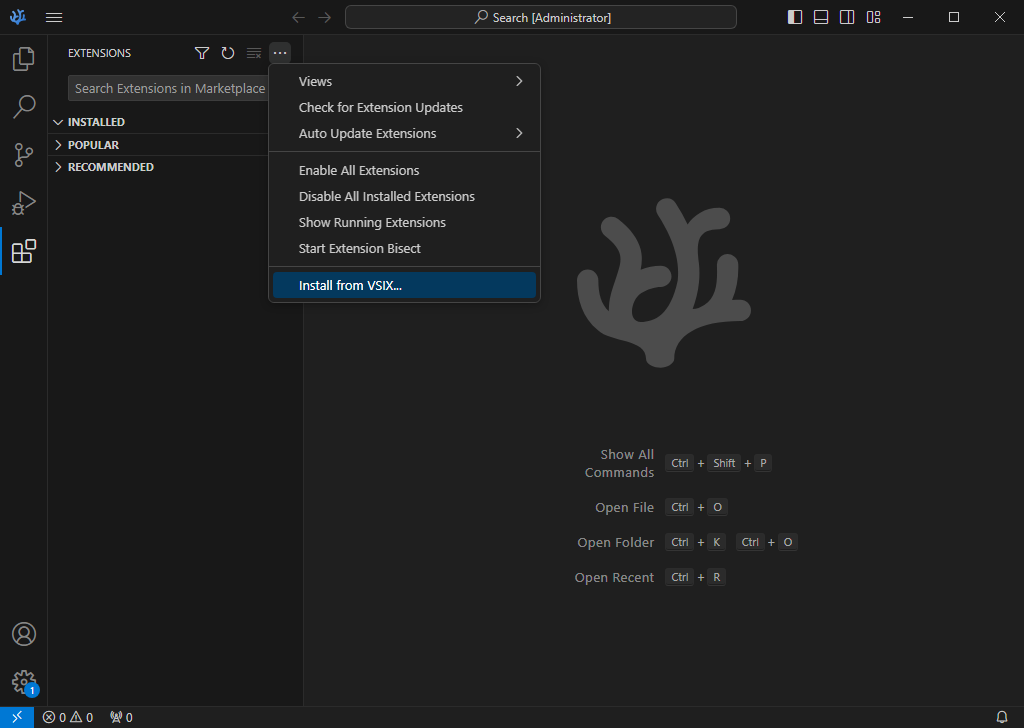
\includegraphics[width=0.85\textwidth]{images/Installing_downloaded_extensions.png}
			\caption {Установка скачанных расширений}
            \label{fig:installing_downloaded_extensions}
        \end{figure}
        
        
        \subsection{ Настройка параметров VSCodium}
        
        Зайдите в настройки, например, с помощью комбинации клавиш Ctrl+, (эту запятую не так просто увидеть) и измените параметр \textquotedbl cmake.cmakePath\textquotedbl \ (этот параметр можно написать в строке поиска для быстрого поиска) на следующий \textquotedbl C:\textbackslash msys64\textbackslash mingw64\textbackslash bin\textbackslash cmake.exe\textquotedbl (см. рис.~\ref{fig:Settings_of_interface})\ или добавьте в файл \textquotedbl settings.json\textquotedbl \ следующую строку (см. рис.~\ref{fig:Settings_of_json_file}):

        \textquotedbl cmake.cmakePath\textquotedbl: \textquotedbl C:\textbackslash\textbackslash msys64\textbackslash\textbackslash mingw64\textbackslash\textbackslash bin\textbackslash\textbackslash cmake.exe\textquotedbl,
    
        Обратите внимание, что если выбрана вкладка User, то изменяются настройки для пользователя, т.е. для всех проектов, а если выбрана вкладка Workspace, то только для текущего проекта и изменения вносятся в файл \textquotedbl .vscode/settings.json\textquotedbl.
        
        Примечание. 
        В интерфейсе VSCodium и в файле \textquotedbl settings.json\textquotedbl \ с настройками \textbackslash ~(backslash) отображается по-разному.
        
        \begin{figure}[H]
            \centering
			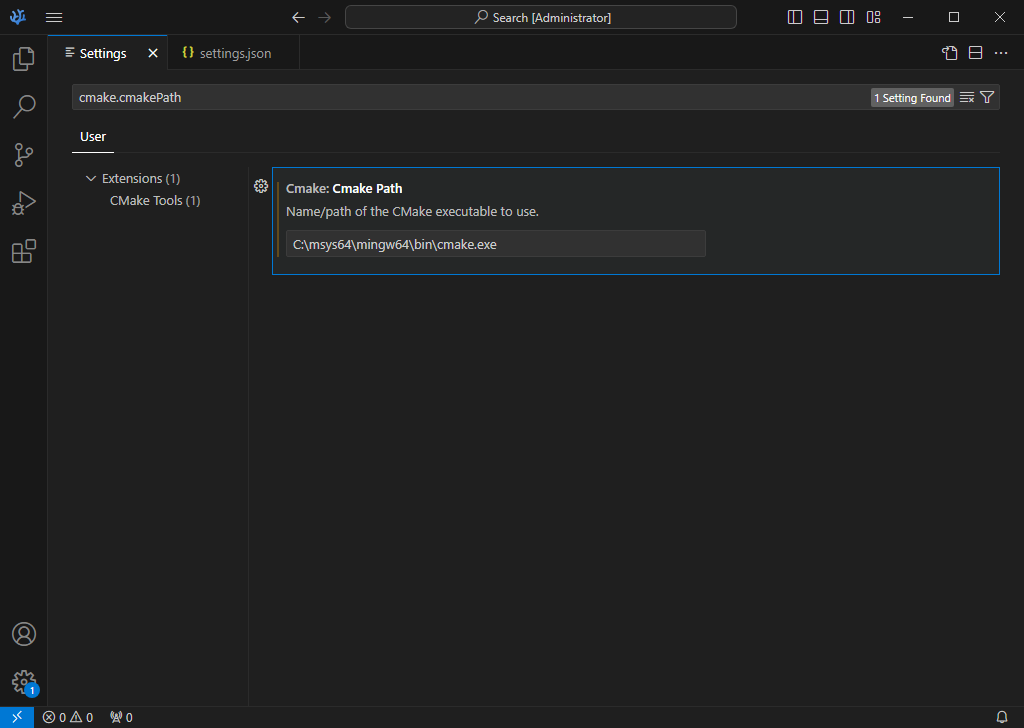
\includegraphics[width=0.85\textwidth]{images/Settings_of_interface.png}
			\caption {Изменение настроек с помощью интерфейса}
            \label{fig:Settings_of_interface}
        \end{figure}
        
        \begin{figure}[H]
            \centering
			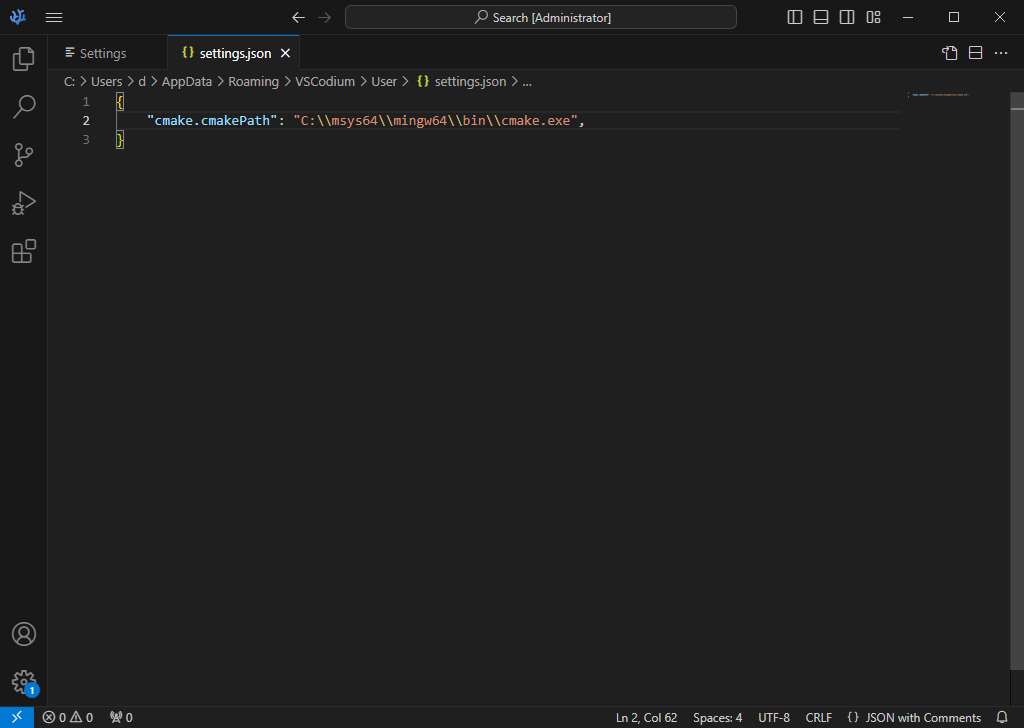
\includegraphics[width=0.85\textwidth]{images/Settings_of_json_file.png}
			\caption {Изменение настроек в файле \textquotedbl settings.json\textquotedbl}
            \label{fig:Settings_of_json_file}
        \end{figure}
        
        
        
        \section{ Запуск проекта \textquotedbl P2-Geometric\_primitives\textquotedbl }
        
        Чтобы убедиться, что все работает корректно, осталось лишь скомпилировать и запустить проект.

        Но перед этим откройте в новом окне VSCodium, нажав комбинацию клавиш Ctrl+Shift+N. После нажмите Ctrl+O, и выберете в директорию \\ Practicum/P2-Geometric\_primitives.
        
        Теперь, чтобы использовать файл (.vscode/cmake-kits.json), расположенный в скрытой директории, с прописанными путями к необходимым установленными вами компиляторам,
        выполните комбинацию клавиш Ctrl+Shift+P, выберете
        \textquotedbl >CMake: Select a Kit\textquotedbl
        (см. рис.~\ref{fig:CMake_select_a_Kit}) и сразу из выпадающего списка выберете \textquotedbl gcc and g++\textquotedbl (см. рис.~\ref{fig:CMake_compiler_paths}).
        
        
        
        \begin{figure}[H]
            \centering
			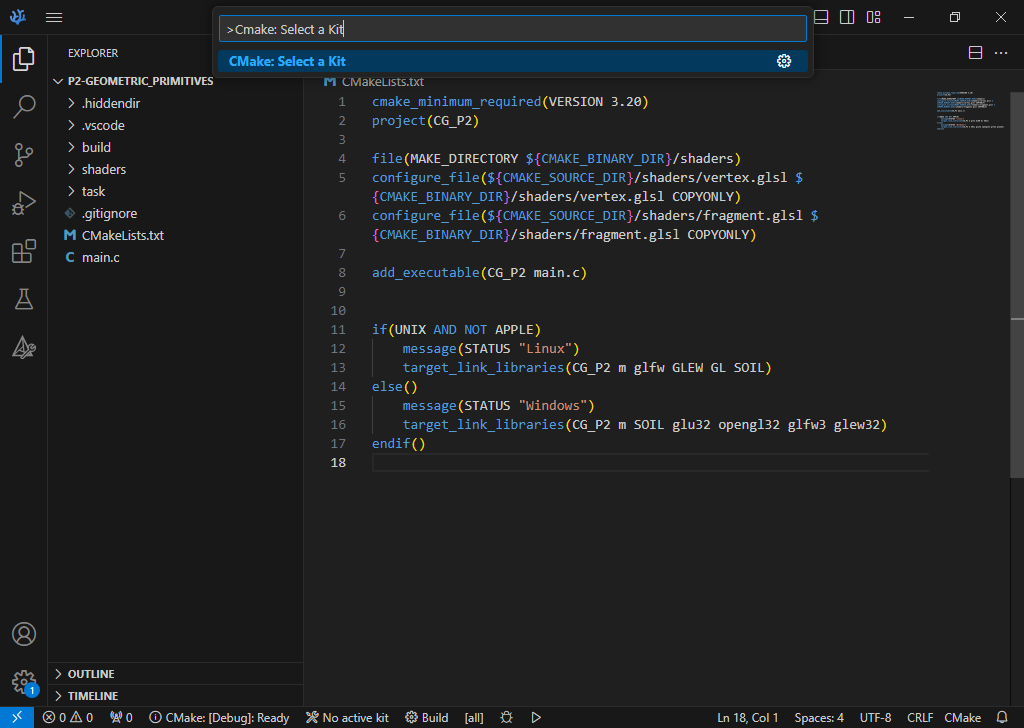
\includegraphics[width=0.85\textwidth]{images/CMake_select_a_Kit.png}
			\caption {Настройка CMake}
            \label{fig:CMake_select_a_Kit}
        \end{figure}

        Примечание.        
        Возможно, могут возникнуть проблемы, если в пути, т.е. адресе директории, куда скопирован ваш репозиторий https://github.com/sci-d3v/CG.git, содержатся русские символы.
        
        
        
        \begin{figure} [H]
            \centering
			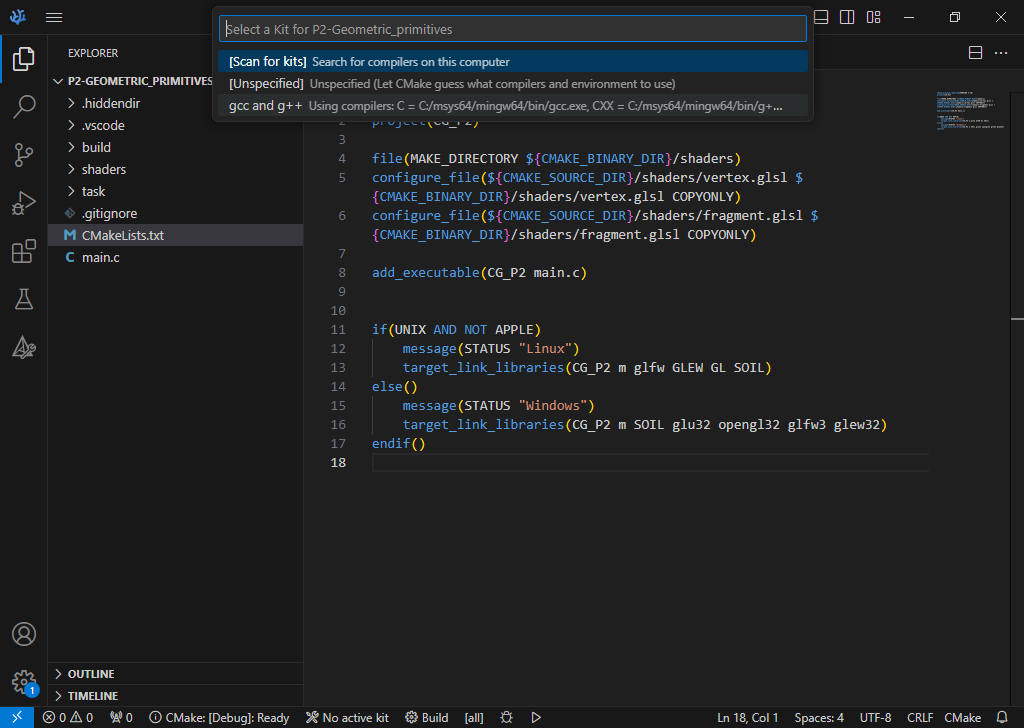
\includegraphics[width=0.85\textwidth]{images/CMake_compiler_paths.png}
			\caption {Возможные варианты путей к компиляторам для CMake}
            \label{fig:CMake_compiler_paths}
        \end{figure}

        Откройте файл CMakeLists.txt и сохраните его, нажав Ctrl+S, при этом произойдет автоматическая сбока или пересборка проекта.

        \begin{figure} [H]
            \centering
			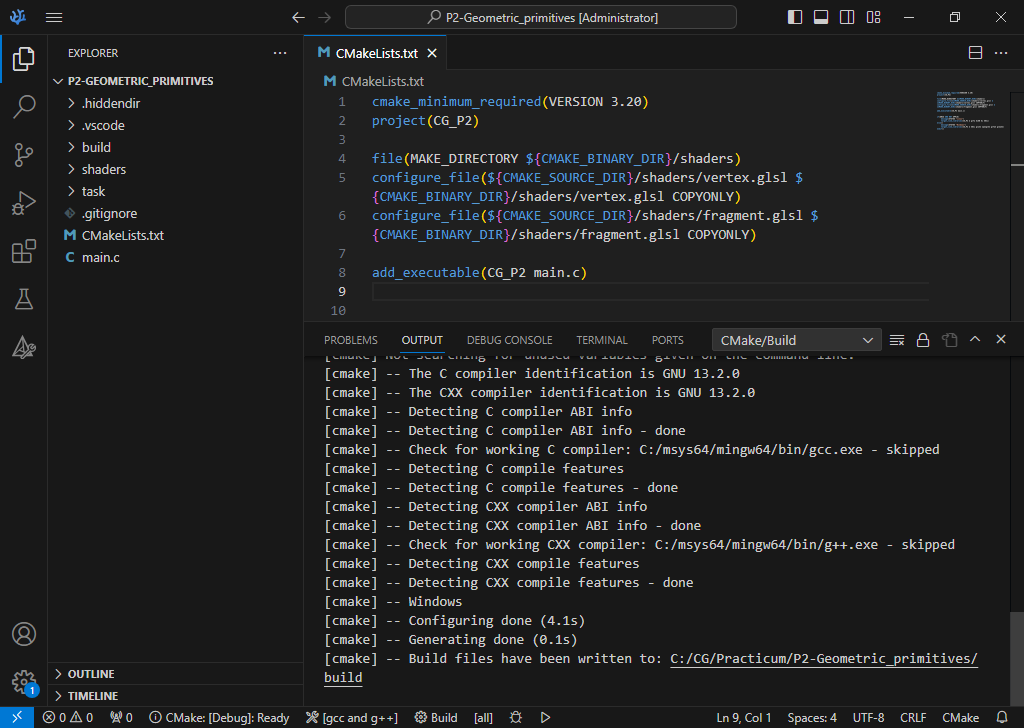
\includegraphics[width=0.85\textwidth]{images/CMake_build.png}
			\caption {Возможные варианты путей к компиляторам для CMake}
            \label{fig:CMake_build}
        \end{figure}
        
        Теперь можно компилировать и запустить собранное приложение \textbf{либо} с помощью комбинаций клавиш Ctrl+Shift+P и прописыванием команд, например,  \textquotedbl>CMake: Build\textquotedbl, \textquotedbl >CMake: Debug\textquotedbl и т.д., \textbf{либо} с помощью интерфейса небольшой панели (синей), расположенной в нижней части ИСР VSCodium.

\end{document}

